% !BIB TS-program = biber
\documentclass[11pt, letterpaper]{article}
\usepackage[letterpaper, margin=1in]{geometry}
\usepackage{graphicx}

\usepackage{caption}
\usepackage{subcaption}

\usepackage{sidecap}  %required for side captions
\usepackage{enumitem}
\usepackage{amsmath}
\usepackage[colorlinks=true, allcolors=black]{hyperref}
\usepackage{setspace}
\usepackage{url}
% here for H placement parameter
\usepackage{float} 
% itemize with custom description labels
\usepackage{blindtext}
\usepackage[english]{babel}
\usepackage{multirow}
\usepackage[toc,page]{appendix}
\usepackage{verbatim}
%% quoting ...
\usepackage{csquotes}% Recommended
% quote to spec
\newcommand{\xquote}[1]{\begin{displayquote}\enquote*{#1}\end{displayquote}}
%biblio, Harvard styling
\usepackage[style=authoryear,maxitems=1, maxcitenames=1, backend=biber]{biblatex}
\renewcommand*{\nameyeardelim}{\addcomma\space}
% line spacing
\renewcommand{\baselinestretch}{1.5}
% ruled line for title 
\newcommand{\HRule}{\rule{\linewidth}{0.5mm}}
\newcommand{\impl}{$\implies$}
%Import the bibliography file
\addbibresource{ref.bib} 
% path to figures
\graphicspath{{figs/}}

%%%%%%%%%%%%%%%%%%%%%%%%%%%%%%%%%%%%%%%%%%%%%%%%%%%%%%%%%%%%%
\begin{document}
%% to print all bib information, use this ..
\nocite{*}

\begin{titlepage}
\center 
\textsc{\LARGE Imperial College}\\[1.25cm]
\textsc{\Large Business School}\\[0.5cm]
\large Work Study Report\\[1.5cm] 
\HRule \\[0.3 cm]
{\huge \bfseries Sentiment Analysis and Topic Modeling of Customer Reviews to understand and improve product quality and process}\\% Title of your document
\HRule \\[0.5cm]
{\large \textbf \\ Author: Bharath Mukundakrishnan}
{\large \textbf \\ Prepared for\\ MiComp Soultions Inc. \\\tiny \textit{(An Agile Health Company)}\\\large Agile Health Technologies Inc.\\2728 Forgue Drive, Suite 106 Naperville, IL-60564} 
{\large \today }\\[2cm] % Date, change the \today to a set date if you want to be precise
\begin{center}
 \begin{tabular}{||c c||} 
 \hline
 \textbf{Student Name} & \textbf{CID} \\
 \hline\hline
 Barry Mukundakrishnan & 01901006 \\ [0.5ex] 
 \hline
\end{tabular}
\end{center}
\vfill
Word Count: 2740
\vfill 
\end{titlepage}

\section*{Executive Summary}
Contact lenses, as an alternative to normal glasses, are used widely and offers many advantages. It is discreet, not subject to misplacement and offer aesthetic advantages that cannot be matched by normal glasses. However, since the lenses are worn on top of the iris, the quality of glass, the material of glass is quite important for customers to feel comfortable. Thus it is important for manufacturers of contact lenses to understand the sentiment(s) of people wearing these lens, regarding the lens. Given the popularity of contact lenses over normal glasses, it is no surprise that there are various companies manufacturing them. There are also various brands of lenses manufactured by the same company in many cases. This study aims to model customer sentiments and automatically extract general discussion topics based on the reviews of contact lenses manufactured by Johnson \& Johnson Inc. The result of the study will be used to see if there are trends and patterns in the usage of these lenses. The extracted discussion topics will allow the manufacturers of lenses to understand if there are issues in the product that needs to be addressed. We plan to use machine learning methods to study the customer review data, predict customer sentiments and extract discussion topics from reviews. We present the model and results from such endeavor.
 

\newpage
\tableofcontents
\newpage

\section {Introduction}
In this project, we model customer sentiment and extract topics of discussion ('topic modeling') from customer reviews of various contact lens brands. The company for which the project was undertaken wants to know how users are responding to their contact lens models on sale. Sample, time ordered customer reviews (8794 data points over 3 months) were provided to us by the customer to establish learning models. This will then be applied over a larger dataset in production. The company is interested in knowing:
\begin{enumerate}
    \item Sentiment of the customer upon buying and usage of the product (Positive, neutral and negative sentiment)
    \item A way to automatically extract discussion topics embedded in customer reviews \label{topicmodeling}
\end{enumerate}
Particularly, the company is interested in understanding if people are discussing about the price, service, and quality of the product. This will help the company to rectify any issues and to know what works and what does not in their products. We use Natural Language processing (NLP) techniques and ML techniques to determine sentiments and do topic modeling.

\section{Introduction to NLP}
Natural Language Processing (NLP) is the processing and generation of language used for communication by humans. Broadly, there are two components to any language: the syntax (structure) and the semantics of the words used in communication. While it is relatively easier to "algorithmize" the structure of the language, it is extremely difficult to extract semantics from text. NLP attempts to understand the meaning of sentences. We use NLP techniques to extract semantics from customer reviews. We use various ML methods, dictionary methods including Neural Network models (RNN) towards this purpose.

\section {Exploratory Data Analysis}
Each row in the input data is one single review of a customer about a brand of contact lens, at a specific date. The fields of input data (Figure \ref{fig:input}) are:
\begin{figure}[H]%
    \centering
    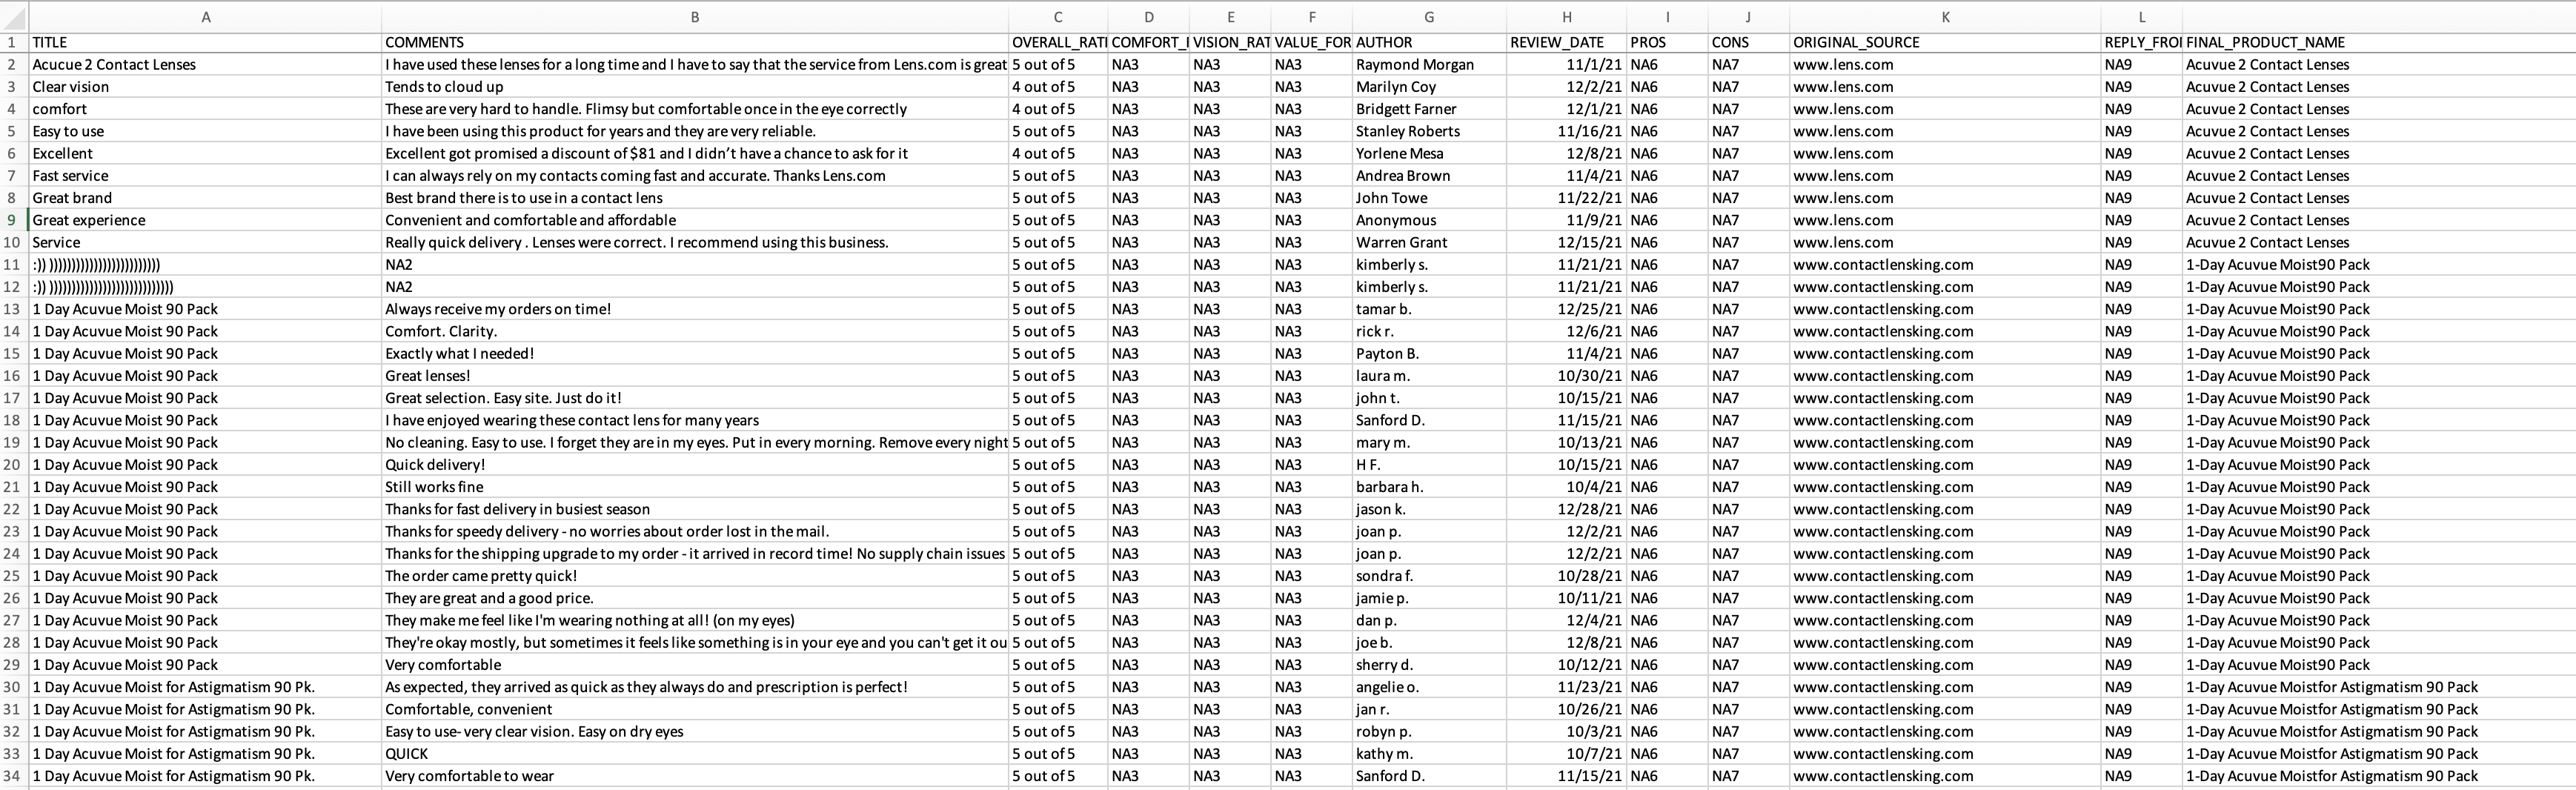
\includegraphics[width=\linewidth]{raw_data.png}%
    \caption{Input customer data}%
    \label{fig:input}
\end{figure}
\subsection {Data pre-processing}
\subsubsection{Input Fields Description}
The various fields available in the input are: 
\begin{verbatim}
'TITLE', 'COMMENTS', 'OVERALL_RATING', 
'COMFORT_RATING', 'VISION_RATING', 'VALUE_FOR_MONEY', 
'AUTHOR', 'PROS', 'CONS', 'ORIGINAL_SOURCE', 
'REPLY_FROM_ACCUVUE', 'FINAL_PRODUCT_NAME', 
'PRODUCT_LINK', 'WEBSITE', 'RATING', 'PRODUCT', 'BRAND'
\end{verbatim}

The columns that are important for our analysis are:
\begin{itemize}
    \item \verb|REVIEW_DATE| The date of the comment. 
    \item \verb|TITLE| The title of the comment, if any. Customers sometimes leave comments in title
    \item \verb|COMMENTS| The comments data on which we need sentiment analysis to be done
    \item \verb|RATING| This is the response variable that "trains" our sentiment analysis algorithm
    \item \verb|PRODUCT| The name of the product 
    \item \verb|BRAND|   Brand of the product
    \item \verb|AUTHOR|  The name of the commentator
\end{itemize}
The comments are found both in the 'TITLE' or in the 'COMMENTS" and so these two are consolidated into one field. Further we extract gender data from names provided and add it to the data. 

\subsubsection{Mean Ratings to understand user Sentiment}
We want to understand the mean ratings of the customers, a proxy for sentiments. This will help in tuning various parameters of sentiment analysis using sophisticated ML models.
\begin{figure}[H]%
     \centering
     \begin{subfigure}[b]{0.3\textwidth}
         \centering
         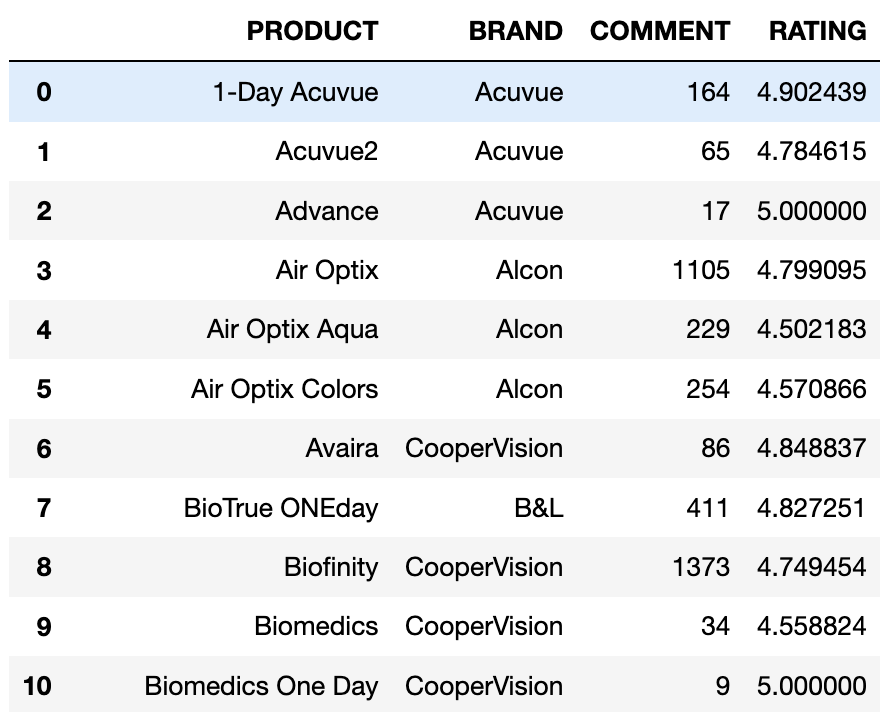
\includegraphics[width=\textwidth]{eda_by_product_brand.png}
         \caption{By product, brand of contact lens}
         \label{fig:bY_product_brand}
     \end{subfigure}
     \hfill
     \begin{subfigure}[b]{0.3\textwidth}
         \centering
         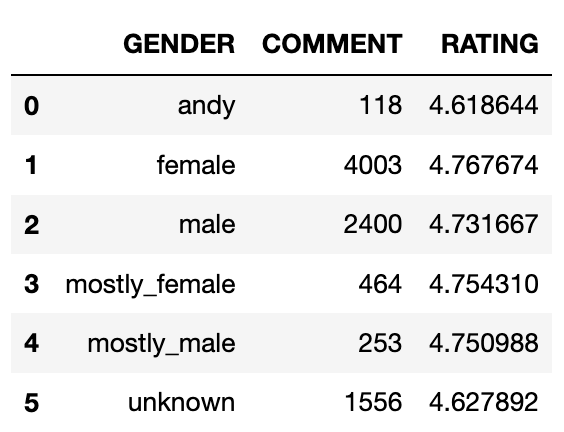
\includegraphics[width=\textwidth]{eda_by_gender.png}
         \caption{By gender}
         \label{fig:by_gender}
     \end{subfigure}
     \hfill
     \begin{subfigure}[b]{0.3\textwidth}
         \centering
         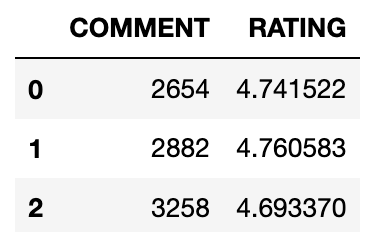
\includegraphics[width=\textwidth]{eda_by_month.png}
         \caption{By month to month}
         \label{fig:by_month}
     \end{subfigure}
        \caption{Mean Review Rating}
        \label{fig:Review rating by various groups}
\end{figure}
We want to understand customer ratings based on the use of words such as "Price, Quality, Service", which help determine if the ratings are influenced by words shown above. We need to 'tokenize' the input reviews. See the following Section \ref{tokenization}.
\begin{figure}[H]%
\centering
\begin{subfigure}[b]{0.45\textwidth}
     \centering
         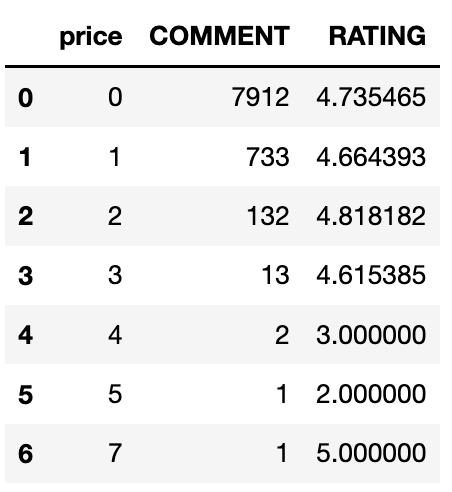
\includegraphics[width=\textwidth]{eda_by_price.png}
         \caption{When using word 'price'}
         \label{fig:eda_by_price}
\end{subfigure}
\hfill
\begin{subfigure}[b]{0.45\textwidth}
         \centering
         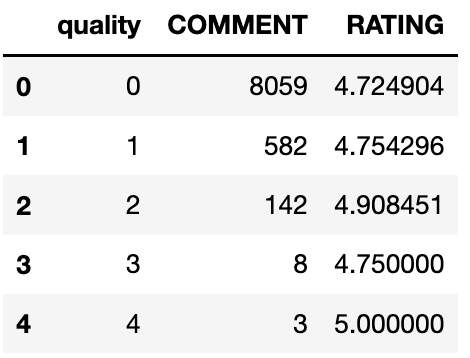
\includegraphics[width=\textwidth]{eda_by_quality.png}
         \caption{When using word 'quality'}
         \label{fig:eda_by_quality}
\end{subfigure}
         \caption{Mean review rating}
         \label{fig:eda_review_rating_demographics}
\end{figure}
%%
\begin{figure}[H]  
\centering
\begin{subfigure}[b]{0.45\textwidth}
         \centering
         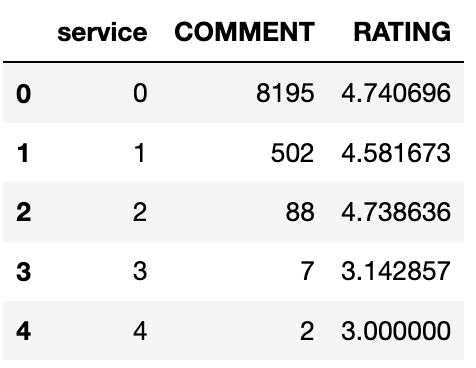
\includegraphics[width=\textwidth]{eda_by_service.png}
         \caption{When using word 'service'}
         \label{fig:eda_by_service}
\end{subfigure}
\hfill
\begin{subfigure}[b]{0.45\textwidth}
         \centering
         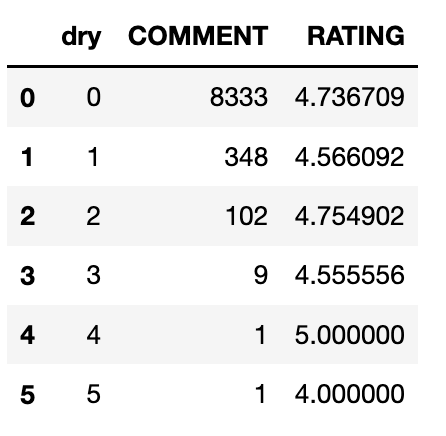
\includegraphics[width=\textwidth]{eda_by_dry.png}
         \caption{When using word 'dry'}
         \label{fig:eda_by_dry}
\end{subfigure}
         \caption{Mean review rating}
         \label{fig:eda_review_rating_words}
\end{figure}

We observe that the sentiments expressed, based on mean ratings are excellent for this data set (mean ratings > 4.0). However, if we look at the mean ratings for the word 'dry', we see that there is a dip in the overall ratings when people use the word 'dry'. Dryness associated with contact lens is a bad thing and this is clearly reflected in the exploratory data analysis. 

\section{Processing reviews into tokens}
In order to use ML algorithms, we need to break down customer reviews into "tokens" or vocabulary words for standardization, thus allowing NLP to be used on the words. In dictionary methods (part of NLP suite of algorithms), we generate vocabulary of words from our domain (and augment these to an already existing vocabulary), extract frequency of occurrence of words in the comments and use this data for further analysis ('Bag of Words' generation). Note that we have not paid heed to meaning or connections between words. A \textit{Document} as a set of sentences or one sentence. So a document correspond to comment text by the user. Further, a set of documents makes a \textit{corpus}. We define these as we will refer to them frequently hereafter.

\subsection{Tokenization and other Pre-processing steps}\label{tokenization}
\begin{enumerate}
 \item \textit{Tokenization}: Splits a string of text into words based on some delimiter. We use the same regular expressions as we would for parsing a tweet \autocite{tokenization}, for describing a token, for this project. 

\item \textit{Punctuation removal}: Remove punctuation in words like \verb|can't| and expand it into full words for analysis

\item \textit{Stop words removal}: Filter often used prepositions like 'and', 'to', 'not' etc. These are called stop words. We filter them because they carry less information. We also filter swords like ('Accuvue' (product name), 'Lens', 'contacts' etc.) which also don't add any value.

\item \textit{Stemming or Lemmatization} \autocite{lemmatization}, \autocite{porter80}, define the terms as: 
\xquote{...\textit{Stemming} usually refers to a crude heuristic process that chops off the ends of words in the hope of achieving this goal correctly most of the time, and often includes the removal of derivational affixes.\\
\textit{Lemmatization} usually refers to doing things properly with the use of a vocabulary and morphological analysis of words, normally aiming to remove inflectional endings only and to return the base or dictionary form of a word, which is known as the lemma.
If confronted with the token \textit{saw}, stemming might return just \textit{s}, whereas lemmatization would attempt to return either \textit{see} or \textit{saw} depending on whether the use of the token was as a verb or a noun ...}. For this project, we 'lemmatize' the token words. It is slow but more robust than stemming.
\end{enumerate}
The following Figure \ref{fig:tokenization} shows the results of pre-processing steps to generate tokens from words.
\begin{figure}[H]%
    \centering
    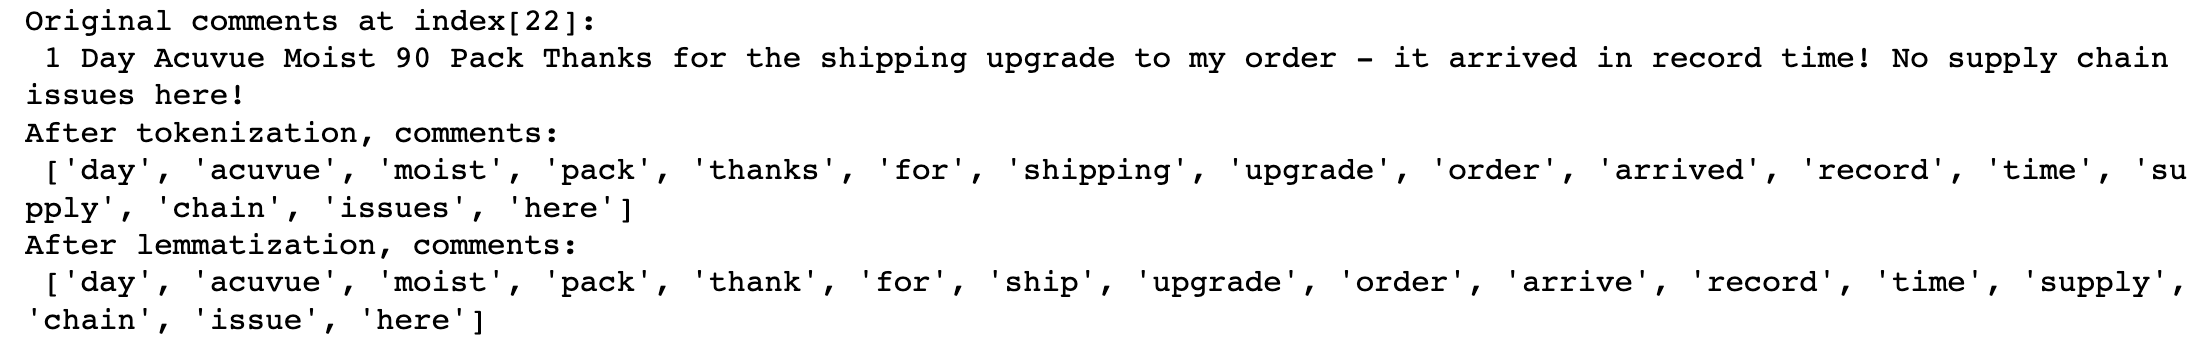
\includegraphics[width=\linewidth]{tokenization.png}%
    \caption{Comments before and after tokenization}%
    \label{fig:tokenization}
\end{figure}
Notice how lemmatization has taken care of words like 'shipping' to 'ship'. Also note that stop words like 'the' and punctuation like '!' have been filtered out. Thus we see how the comments have been broken down into 'machine' usable tokens for processing. From now, all analysis will use these processed comments.

\subsection{Bag of words Analysis}
We take the union of all words in all comments and use each word as a \textit{feature} that contributes to sentiments of the users. The frequency of occurrence of words is used as the measure of that feature. So, we need to determine this frequency of words (or features). We use this value to build the \textit{document-term matrix}, where the rows are made of individual user review, the columns are made of the words used by the customer and the value is the measure of frequency of occurrence of word. In supervised modeling, we determine the relation between these features and the sentiment rating provided by the user. Often, it is observed that there is a power law distribution of words (Zipf’s law \autocite{zipfslaw}). We observe the same in our dataset as well (See Figure \ref{fig:zipflaw}). 
\begin{figure}[H]%
     \centering
     \begin{subfigure}[b]{0.45\textwidth}
         \centering
         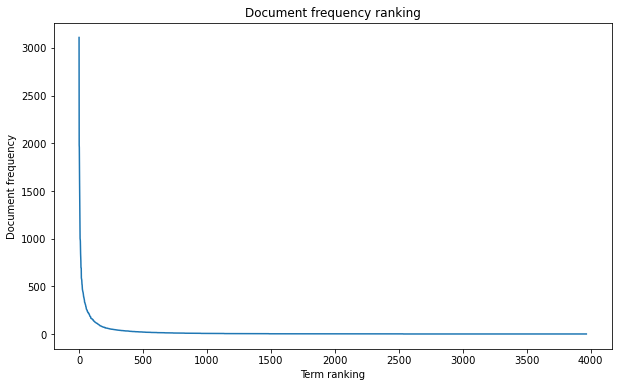
\includegraphics[width=\textwidth]{zipf_law.png}
         \caption{Zipf's law}
         \label{fig:zipflawa}
     \end{subfigure}
     \hfill
     \begin{subfigure}[b]{0.45\textwidth}
         \centering
         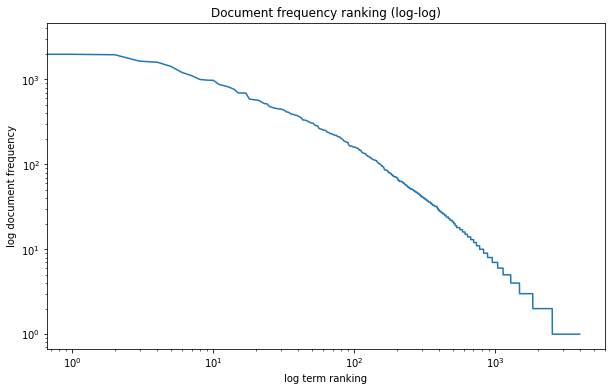
\includegraphics[width=\textwidth]{zipf_log_log.png}
         \caption{Zipf's law log-log plot}
         \label{fig:zipflawloglog}
     \end{subfigure}
        \caption{Word distribution in the entire corpus}
        \label{fig:zipflaw}
\end{figure}
Typically, the word frequency is measured in two common ways:
\begin{itemize}
    \item Term Frequency/Document Frequency (TF/DF)
    \item Term Frequency-Inverse Document Frequency (TF\_IDF)
\end{itemize}
See \autocite{documenttermmatrix}, \autocite{nlpbasics} for details. In this project, we don't use the popular \textit{TF\_IDF} because it seems to highlight tokens that suggest advertising words and use the basic DF method for counting tokens to fill the document-term matrix. See Figure \ref{fig:Word distribution plot} for the word distribution in the dataset. Note the use of advertisement like terms in TF-IDF tokens.
\begin{figure}[H]%
     \centering
     \begin{subfigure}[b]{0.45\textwidth}
         \centering
         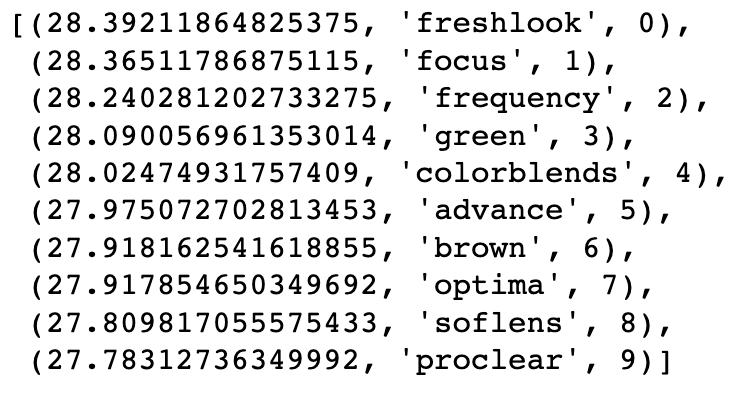
\includegraphics[width=\textwidth]{tfidf.png}
         \caption{TF-IDF based Top tokens}
         \label{fig:tfidf}
     \end{subfigure}
     \hfill
     \begin{subfigure}[b]{0.45\textwidth}
         \centering
         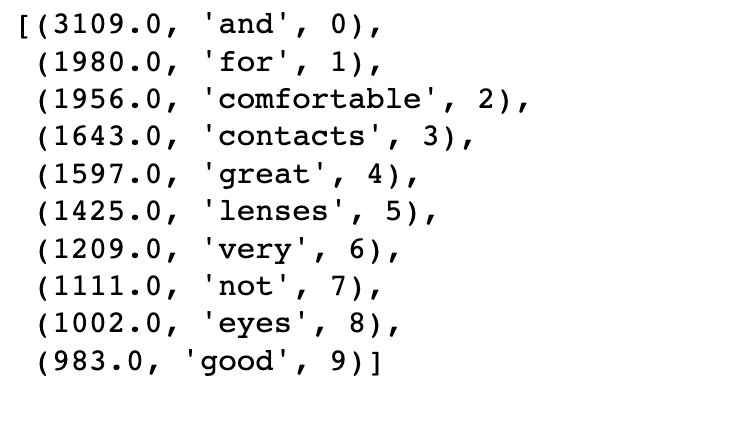
\includegraphics[width=\textwidth]{df_words.png}
         \caption{DF based Top tokens}
         \label{fig:df}
     \end{subfigure}
        \caption{Sorted TF-IDF, DF values of tokens}
        \label{fig:Word distribution plot}
\end{figure}

\section{Sentiment Analysis} 
After creation of document-matrix, the next step is to simplify the \textit{response} variable, the "sentiment" based on user ratings that range from [0-5]. We categorize sentiments into three buckets as:
\begin{itemize}
    \item RATING > 3 \impl \textit{Positive sentiment} [indexed by integer: 2]
    \item RATING = 3 \impl \textit{Neutral sentiment} [indexed by integer: 1]
    \item RATING < 3 \impl \textit{Negative sentiment} [indexed by integer: 0]
\end{itemize}
Supervised ML models can now determine the relationship between the features and sentiments extracted from user ratings. The model thus "learnt" is used as a basis for sentiment analysis on any unknown user comment.

\subsection{Base model}
In a "Base" model, we predict the sentiment using the prior distribution of sentiments in the data without using any other information. This serves as the base model over which to improve upon using other sophisticated ML methods. The results of null model and SVM model are shown in Figure \ref{fig:all_models_confusion}.

%\begin{figure}[H]%
%    \centering
%    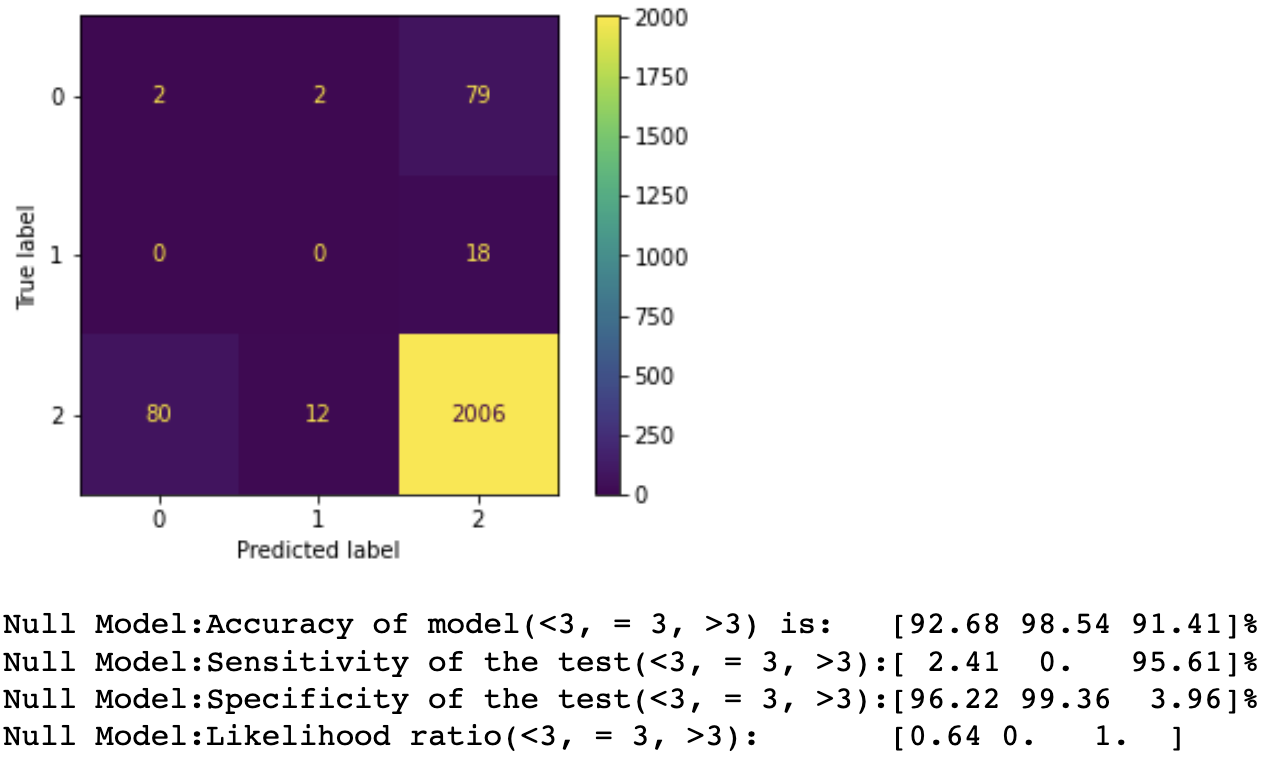
\includegraphics[width=\linewidth]{null_model_metrics.png}%
%    \caption{Metrics of Null model for predicting Sentiments}%
%    \label{fig:null_results}
%\end{figure}

\subsection{Choice of ML model}
While there are many supervised ML models to choose from, we use SVM model in this project. If the idea is to know the probabilities of various sentiments possible in the response, then the simplest ML model to use is the Logistic Regression model. But, if the idea is to make the right decision (i.e., decisions  can be expressed as ratio of likelihoods), then SVM method and logistic regression are similar. Other models such as Naive Bayes, LDA (Linear Discriminant models) assumes class conditional independence, which is not a good assumption for extracting sentiments. Decision tree models are a good choice for this project. But there is no probabilistic distribution assumptions on response fields or feature fields. Further, these models cannot be used in online mode. Hence we use SVM model for our analysis. Even SVM model is not a good model as there is no importance given to word semantics. So, in production, I suggest we use Recurrent Neural Network Model (RNN) for sentiment analysis.

\subsection{Test-Train-Validation split and Data balancing}
We split the dataset into testing, validation and training data for extracting the best ML model. The test-train-validation split has to be done without shuffling the data set as the comments are ordered in time. Further, upon inspection, we see that the sentiment data is highly imbalanced See Figure \ref{fig:imbalanced_data}. This needs to be balanced when applying ML models. We do this by specifying proper weights to models.
\begin{figure}[H]%
    \centering
    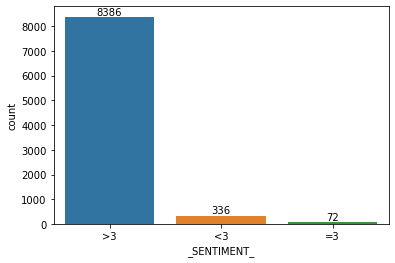
\includegraphics[width=\linewidth]{sentiment_imbalance.png}%
    \caption{Imbalanced sentiment data}%
    \label{fig:imbalanced_data}
\end{figure}

\subsection{Recurrent Neural Network model (RNN) model}
We use LSTM based RNN models (See \autocite{bestrnn}) to incorporate relationship between words written as a sequence (comment statements must be considered as an ordered sequence of words). Further, RNN model uses word embeddings which incorporate semantic meaning of words. Word embeddings \autocite{nlpbasics} encode any word as a vector of unknown but fixed set of features. We use gensim to learn the word embeddings \autocite{gensim}. Training details are found in the code accompanying this report. Here we report the RNN model accuracy estimate (based on test data), convergence of model (based on plot of model loss), See Figures \ref{fig:RNN_model_loss_accuracy}, \ref{fig:all_models_confusion}.

\begin{figure}[H]%
     \centering
     \begin{subfigure}[b]{0.45\textwidth}
         \centering
         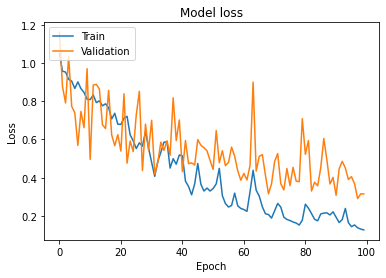
\includegraphics[width=\textwidth]{rnn_model_loss.png}
         \caption{Loss}
         \label{fig:rnn_model_loss}
     \end{subfigure}
     \hfill
     \begin{subfigure}[b]{0.45\textwidth}
         \centering
         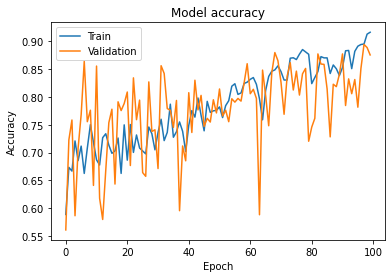
\includegraphics[width=\textwidth]{rnn_model_accuracy.png}
         \caption{Accuracy}
         \label{fig:modelaccuracy}
     \end{subfigure}
        \caption{RNN model's loss function and accuracy on dataset}
        \label{fig:RNN_model_loss_accuracy}
\end{figure}
We can see the convergence as reduction in model loss. We also see that the accuracy is improved as a function of epochs. With more computing power, we should see much better convergence rates.

%\begin{figure}[H]
%         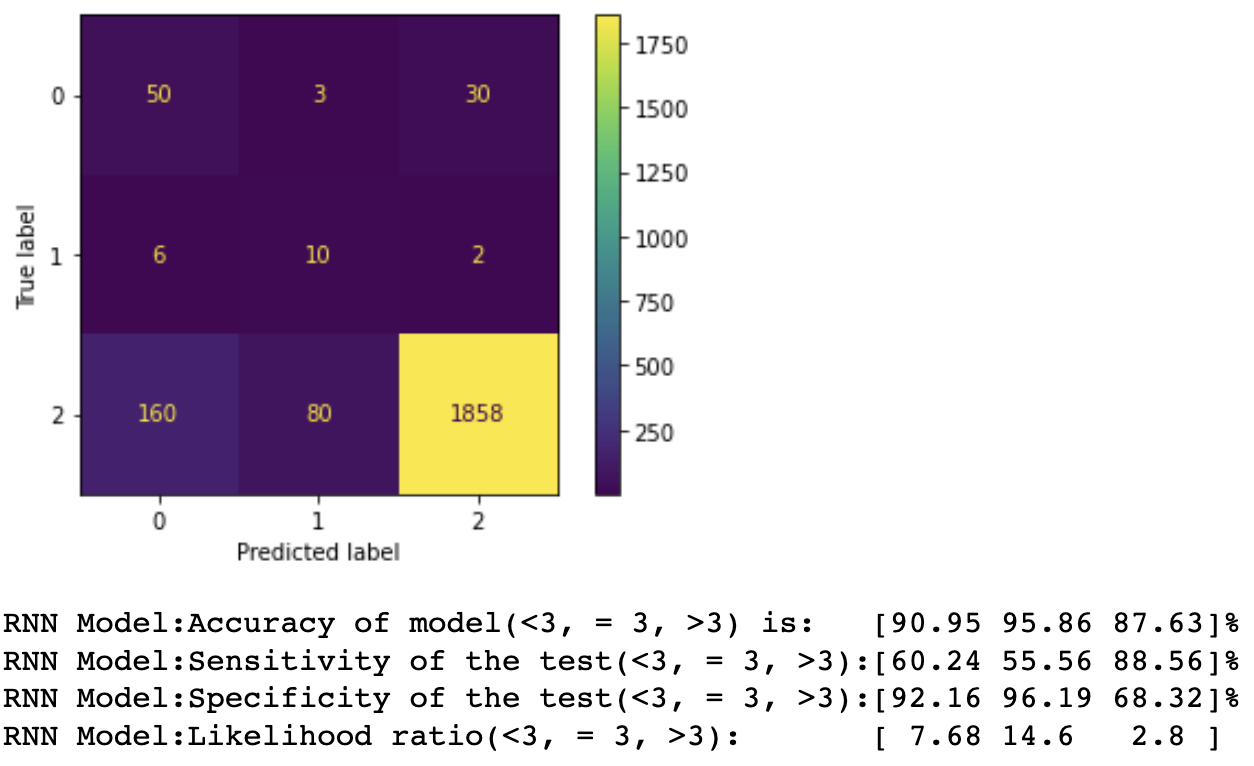
\includegraphics[width=\textwidth]{rnn_model_metrics.png}
%         \caption{Confusion matrix and accuracy metrics of RNN model}
%         \label{fig:rnnconfusionmatrix}
%\end{figure}

\subsection{Consolidated results of supervised Sentiment Analysis}
We present the results of supervised ML models here. 
\begin{figure}[H]%
     \centering
     \begin{subfigure}[b]{0.3\textwidth}
         \centering
         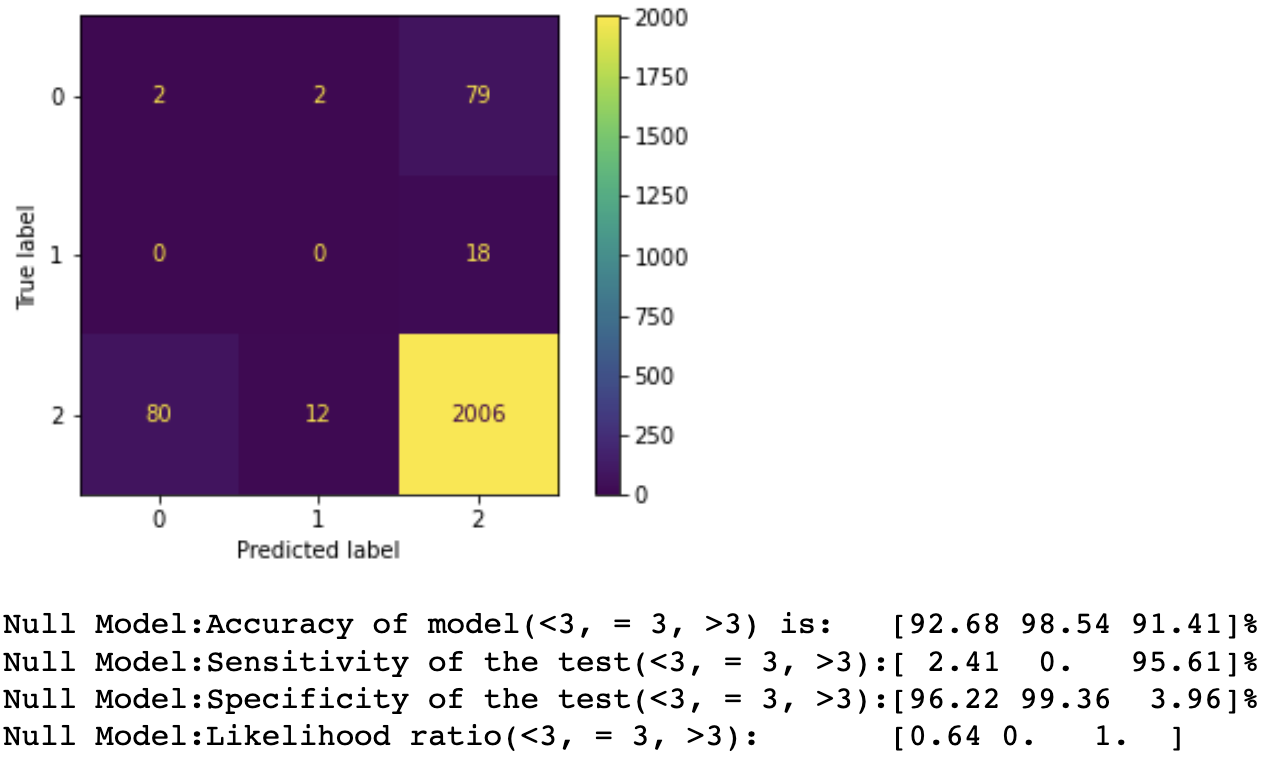
\includegraphics[width=\textwidth]{null_model_metrics.png}
         \caption{Null model}
         \label{fig:Null Model}
     \end{subfigure}
     \hfill
     \begin{subfigure}[b]{0.3\textwidth}
         \centering
         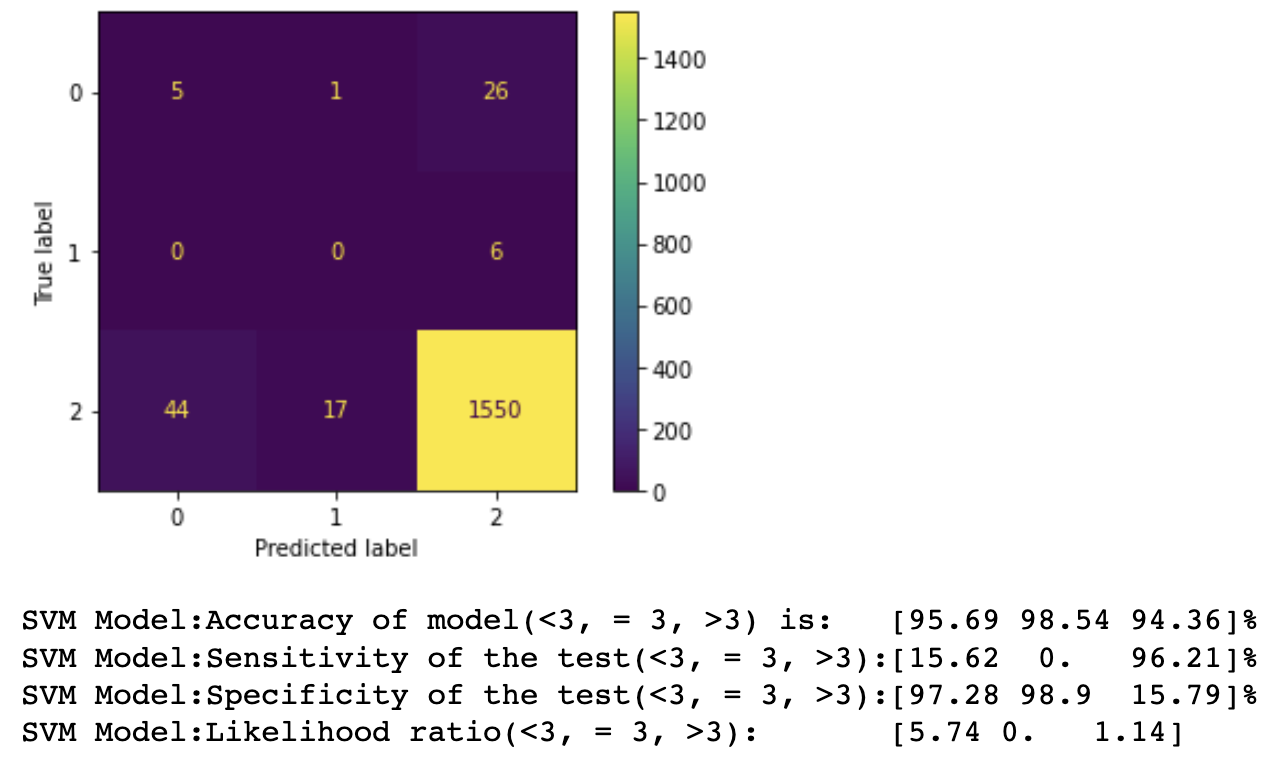
\includegraphics[width=\textwidth]{svm_model_metrics.png}
         \caption{SVM model}
         \label{fig:svm model}
     \end{subfigure}
     \hfill
     \begin{subfigure}[b]{0.3\textwidth}
         \centering
         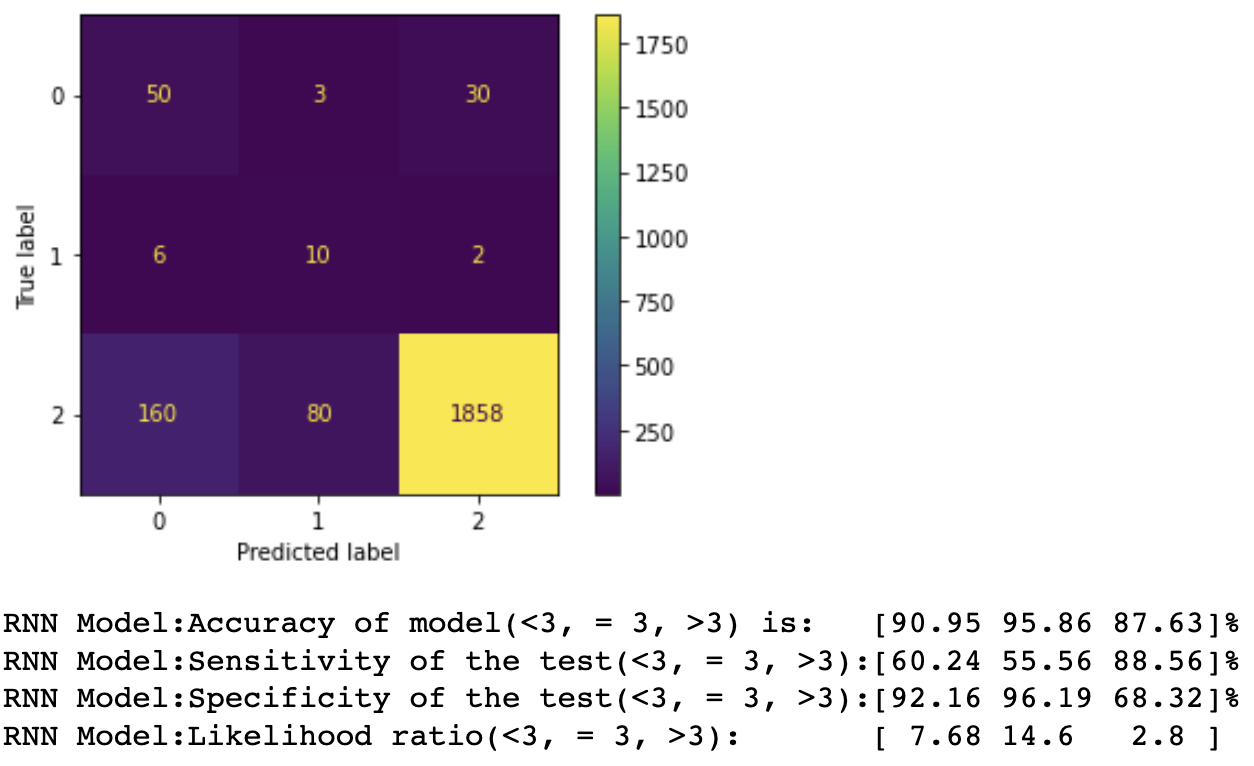
\includegraphics[width=\textwidth]{rnn_model_metrics.png}
         \caption{RNN model}
         \label{fig:rnn kdel}
     \end{subfigure}
        \caption{Confusion matrix \& Metrics of all ML models}
        \label{fig:all_models_confusion}
\end{figure}

\begin{figure}[H]
         \centering
         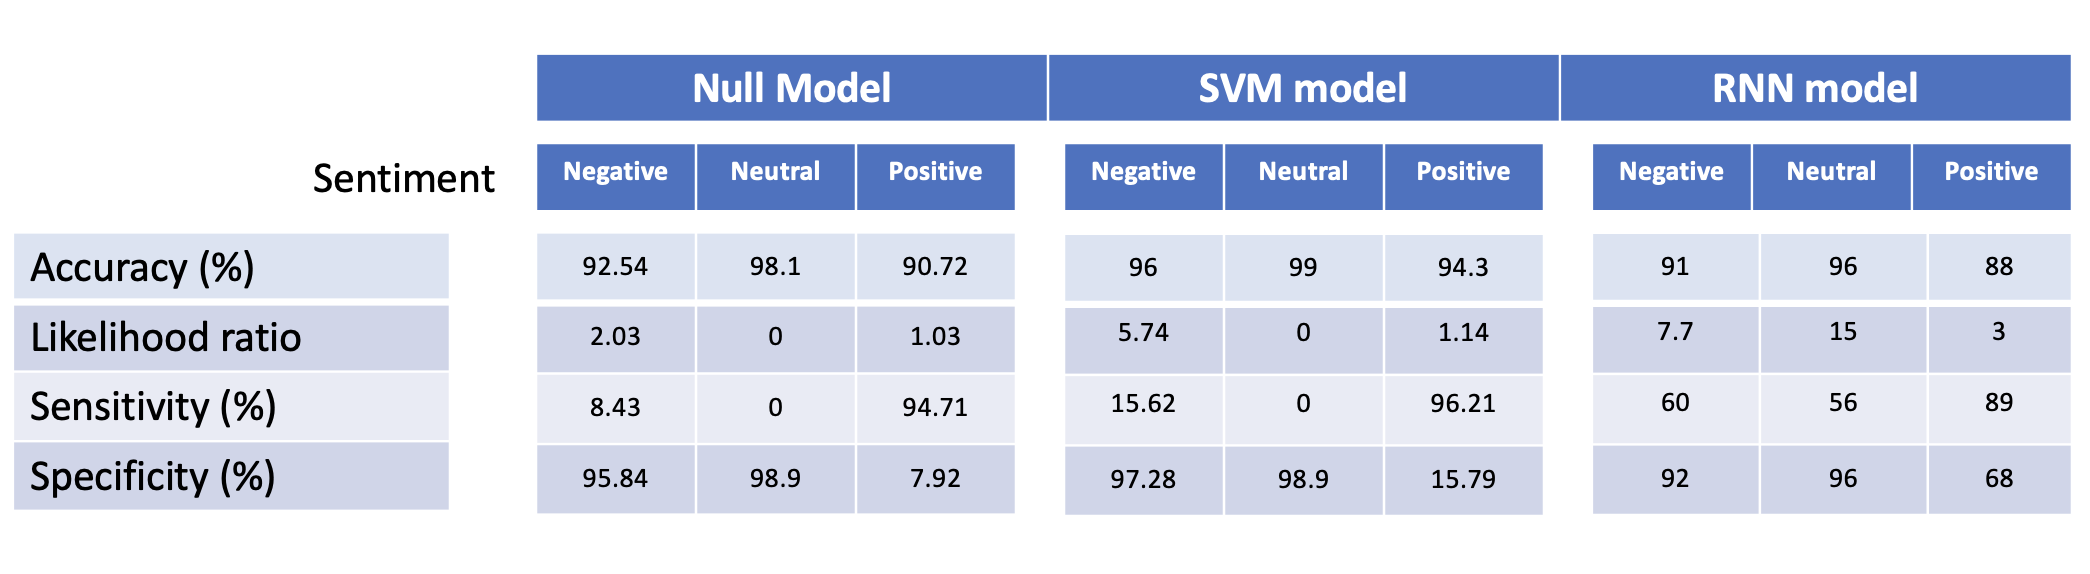
\includegraphics[width=\textwidth]{sentiment_metric.png}
         \caption{Consolidated results of ML models for Sentiment Analysis}
         \label{fig:consolidatedrsults}
\end{figure}

we see that in terms of likelihood ratios, which is the robust measure of assessing a model 
\autocite{uselikelihoods}, RNN model is the best model. Even otherwise, it is the only model that attempts to capture the semantic meaning of comments and needs to be used. 

\section{Topic Modeling using Latent Dirichlet Allocation (LDA) model}
Quite often, one is interested in automatically extracting topics of conversation from a corpus. In this work, for example, the company wants to know what people are discussing considering all the comments as aggregate. Specifically, there are interested to see customer comments on the topics of pricing, quality and service of the product. We use Latent Dirichlet Allocation (LDA) model to determine topics from the corpus.
\subsection{Latent Dirichlet Allocation model}
LDA is that it is a multi-variate expansion of the basic $\beta$-distribution \autocite{betadistribution}, which models proportions of data. In LDA, it is assumed that:
\begin{itemize}
    \item A document is a probability distribution of topics
    \item A topic is a probability distribution of words
\end{itemize}
The idea is to find topics and corresponding word distributions over the topics. The details of LDA model can be found in \autocite{topicmodelinglda}. We present the results, a word cloud of various topics automatically determined from the user comments.
\begin{figure}[H]%
    \centering
    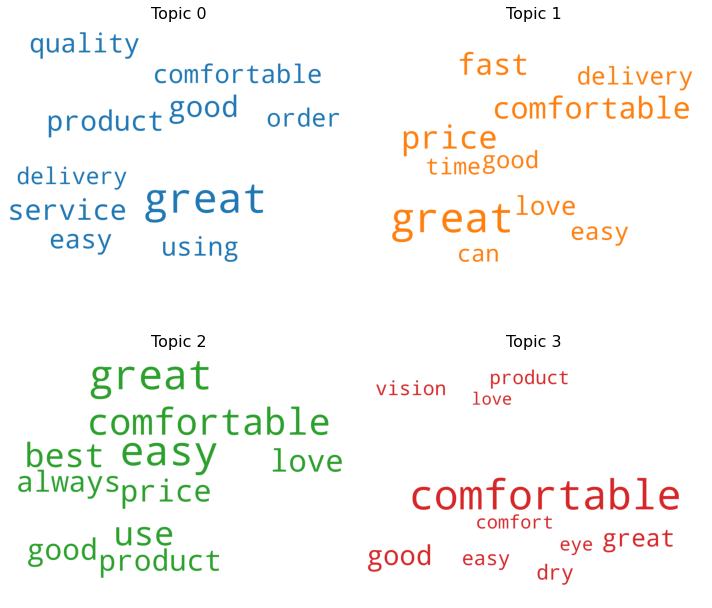
\includegraphics[width=\linewidth]{word_cloud.png}%
    \caption{Word cloud showcasing user comments on different topics}%
    \label{fig:word_cloud}
\end{figure}
The size of the font in the word cloud is proportional to frequency of its occurrence. Note the absence of topic heading. Domain experts can easily understand the headings for the topics. Further, if we look at topic 3 in the word cloud, we see that the word 'dry' showing up prominently. The presence of this word in the topics suggests a problem that the company has to solve. Further, the word cloud also suggest topics that the company should not be worried about, such as the "comfort" level of the lens.

In these following plots, we look at the topics from various points of view.
\begin{figure}[H]%
         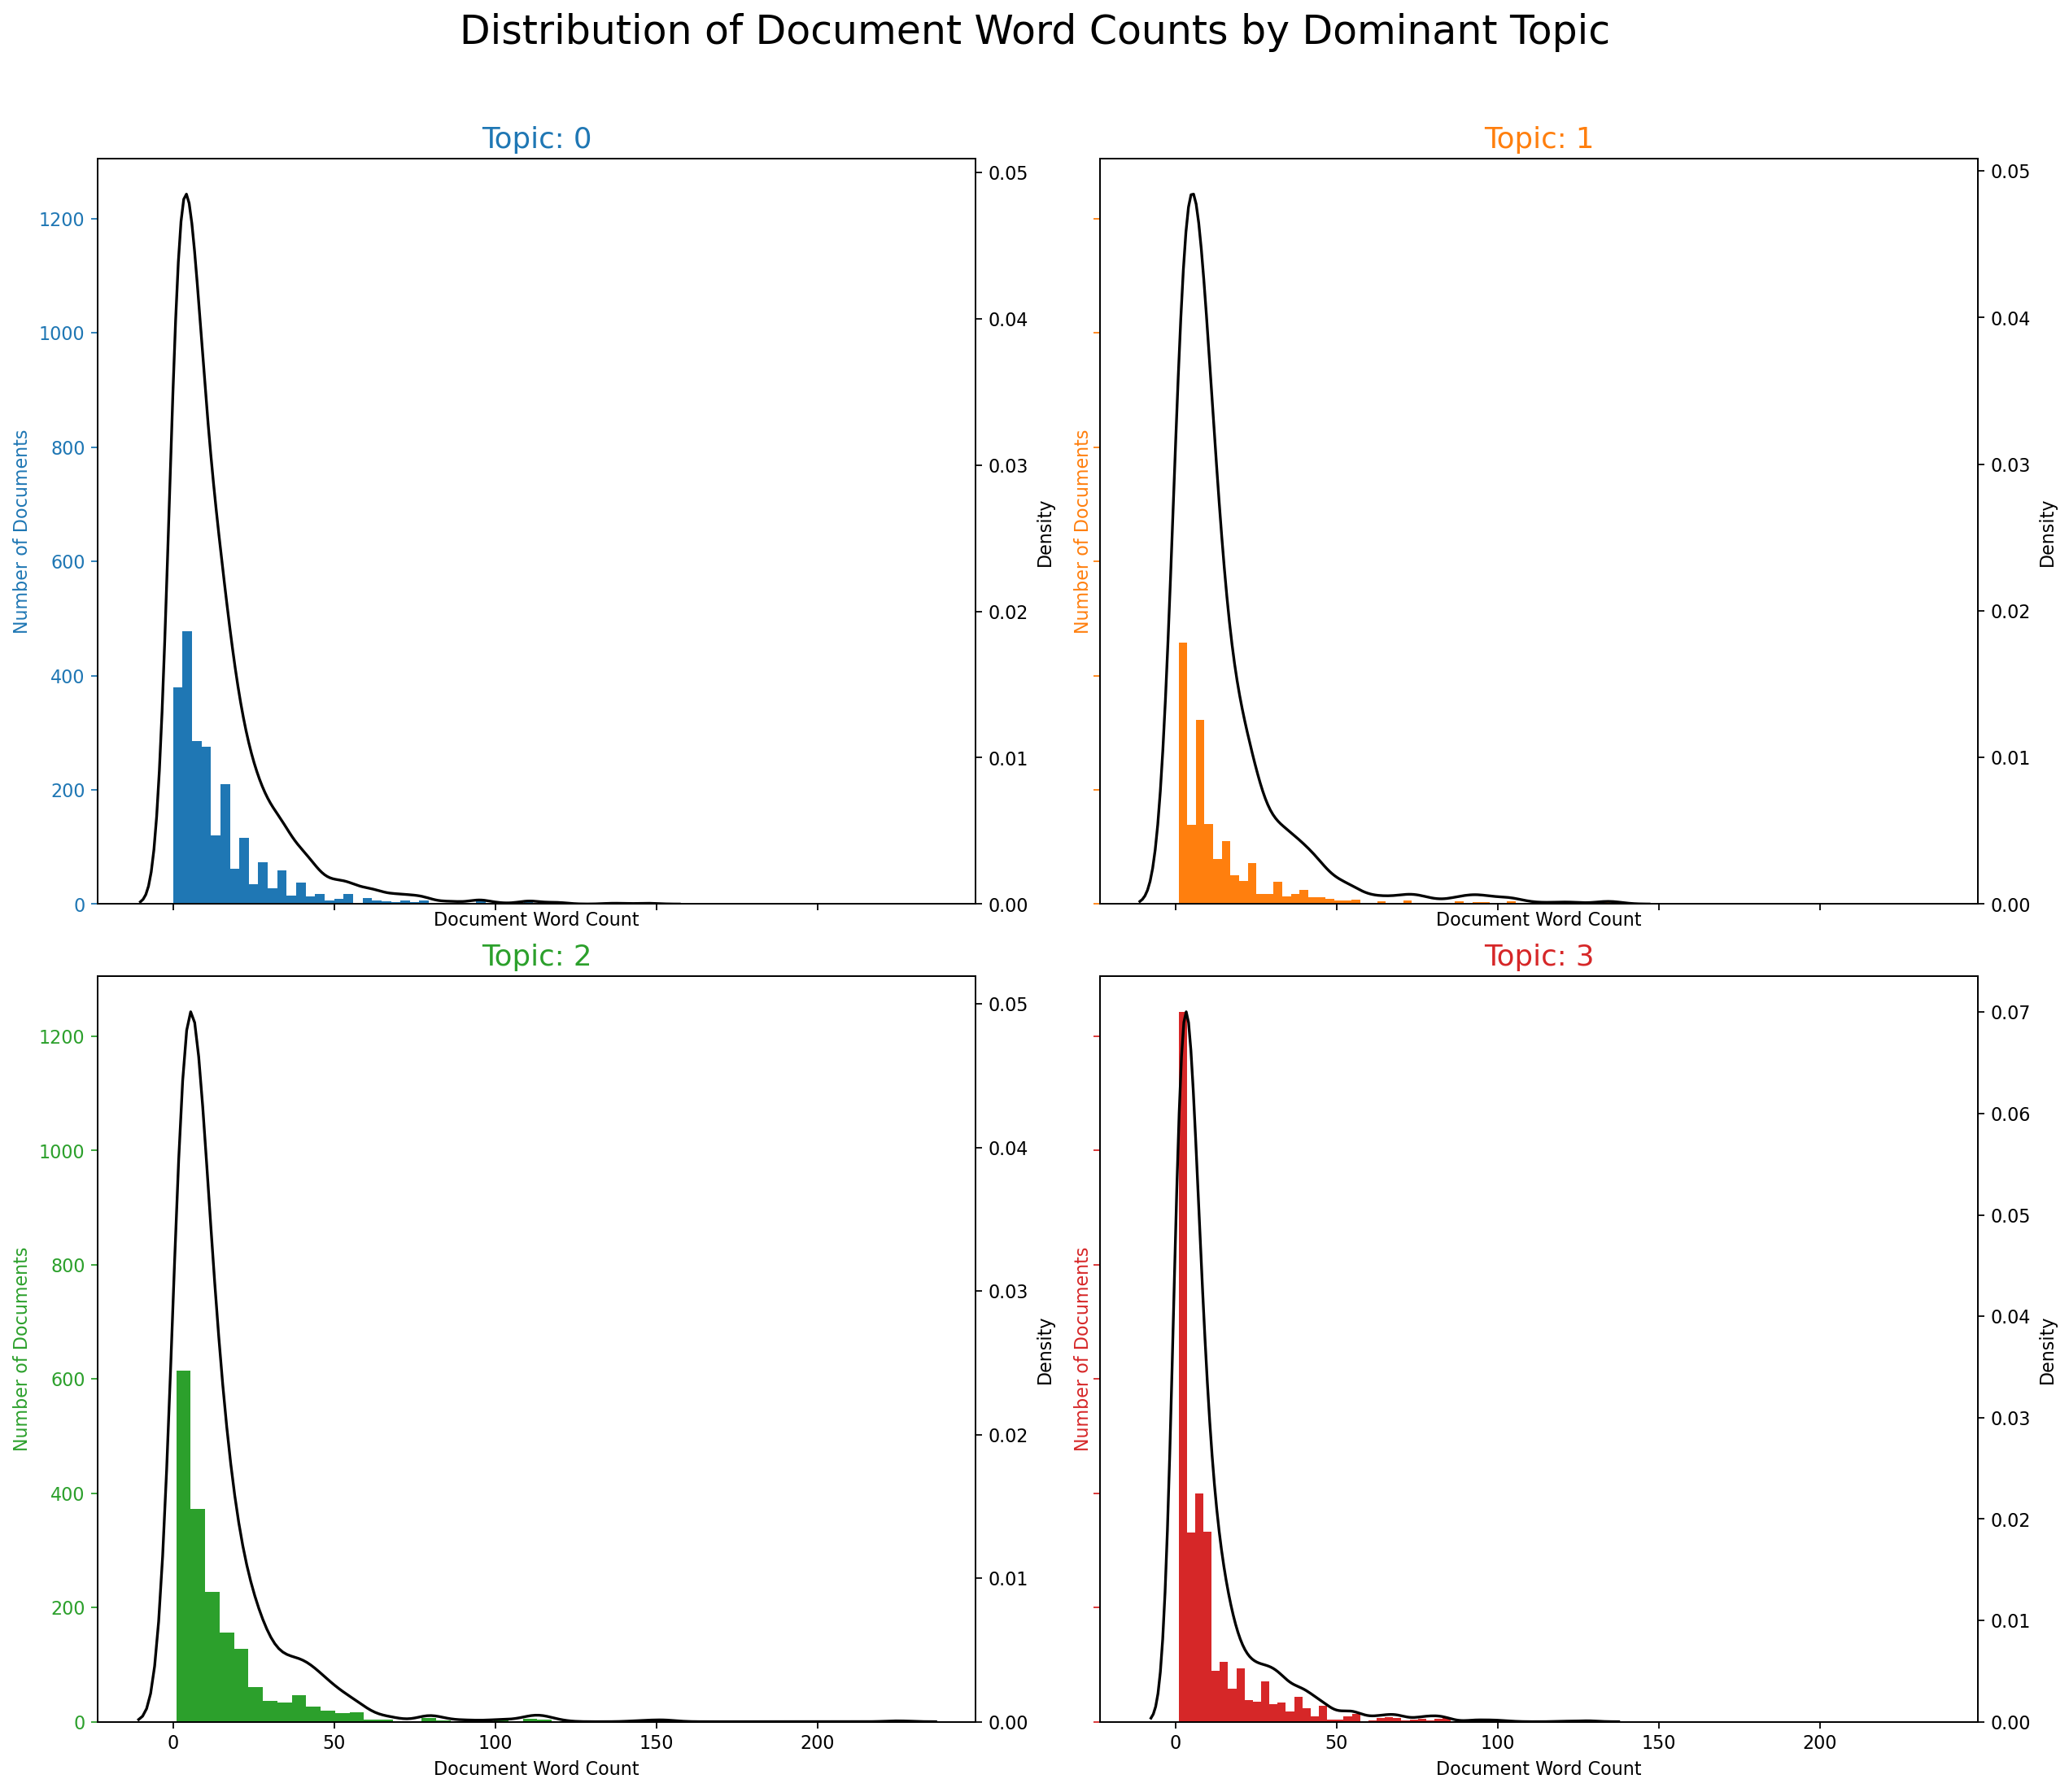
\includegraphics[width=\textwidth]{doc_distribution_by_topic.png}
         \caption{Distribution of documents by topic}
         \label{fig:by_doc_topic}
\end{figure}

\begin{figure}[H]
         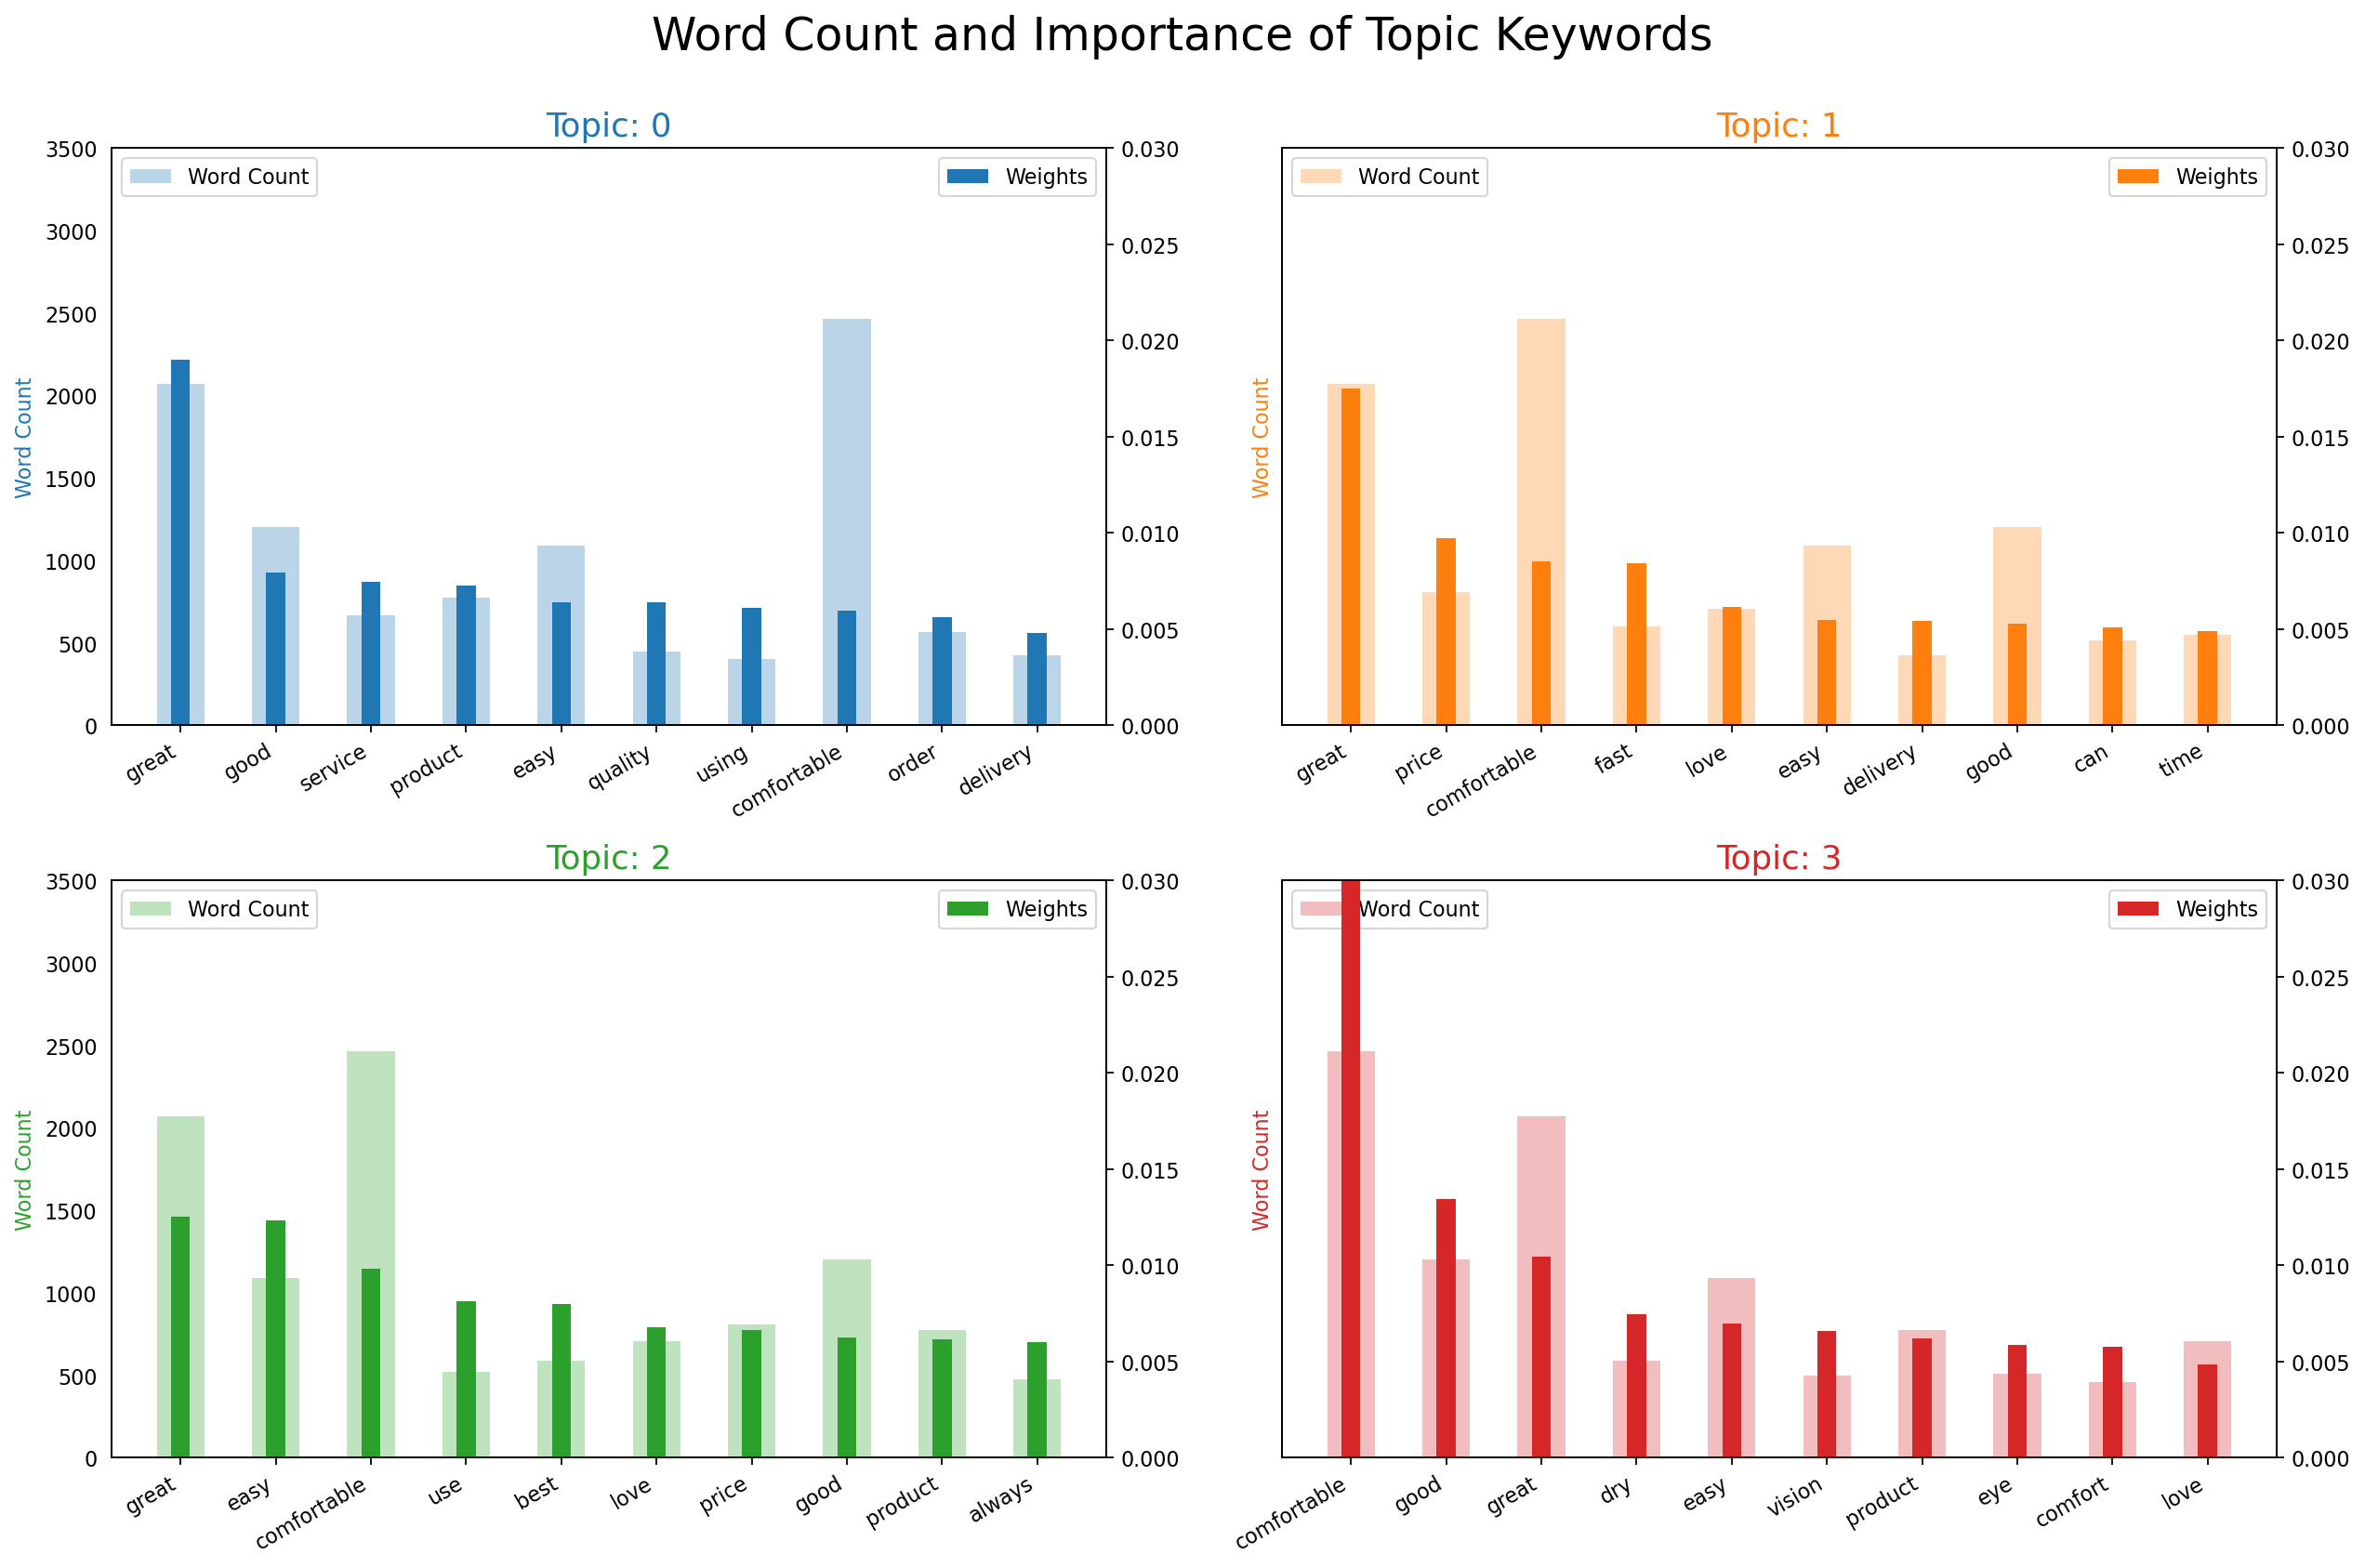
\includegraphics[width=\textwidth]{word_importance_topic.png}
         \caption{Distribution of words over all topics}
         \label{fig:by_word_topic}
     \end{figure}

\subsection{Evaluation of LDA model: Coherence metrics}
How do we know that the LDA model is good?. One standard metric is the "perplexity" metric, i.e. how well the trained LDA model reproduces the statistics of test data \autocite{perplexity}. But it has been found that using a metric called "coherence" metric is much closer to how humans determine topics from words \autocite{topicmodelingcoherence}. This metric evaluates topics based on whether dominant words of the topic are repeatedly used in documents providing a measure of coherence, a measure of semantic meaning to set of words that make up the topic. In this report, we use coherence metric to determine "goodness" of the model. We propose different number of topics and using coherence measure determine the optimal number of different topics embedded in customer reviews. In this dataset, the best coherence measure we obtain is ~0.34 for a total of 4 different topics automatically extracted by the LDA model. Note that the bigger the coherence number, the better is the confidence in topic modeling LDA model. Also note that model automatically splits the data into train-test data internally. 

\section{Conclusions and Recommendations}
We have demonstrated the use of different ML models for sentiment analysis from simple bag-of-words, dictionary methods to sophisticated Neural Network models. Simple ML models ignores the relationship between words, while RNN models takes into account the ordered nature of words in comments and also includes a notion of word semantics. We thus have built up a robust framework for sentiment analysis in this project. Further, we are able to automatically determine topics of discussion given a corpus based on LDA model. Upon discussion with the stakeholders, I would like to report that the topic modeling and word cloud was immediately useful to the customer as they were able to determine that "dryness" seemed to be an issue to be addressed. The next steps are to make this code faster, productize it (including adding user interface) so that it can be deployed by the company.

\section{Limitations and Future Improvement}
We just started the process of sentiment analysis and topic modeling using various ML models in this project. Model tuning and productization will depend on customer needs. I was also limited by the computing power in my desktop and so the search space for model parameters and hyper-parameters were severely limited. We did not explore the latest NLP models (BERT models \autocite{bert}) for sentiment analysis. Further, we did not consider online processing of user data (we did offline batch processing) which would be super useful. Also, we need to present a single unified UI framework for all this work that makes it easier for executives to visualize extracted information. 
\newpage
\printbibliography

\newpage
\begin{appendices}
\section{Principal Component Analysis of Word vector data}
Here we show plot of the result of PCA of word vectors in order to understand the word vectors for our domain and how words (and bi-grams) in our domain are related. The details of the implementation can be found in the HTML file:
\begin{figure}[H]
         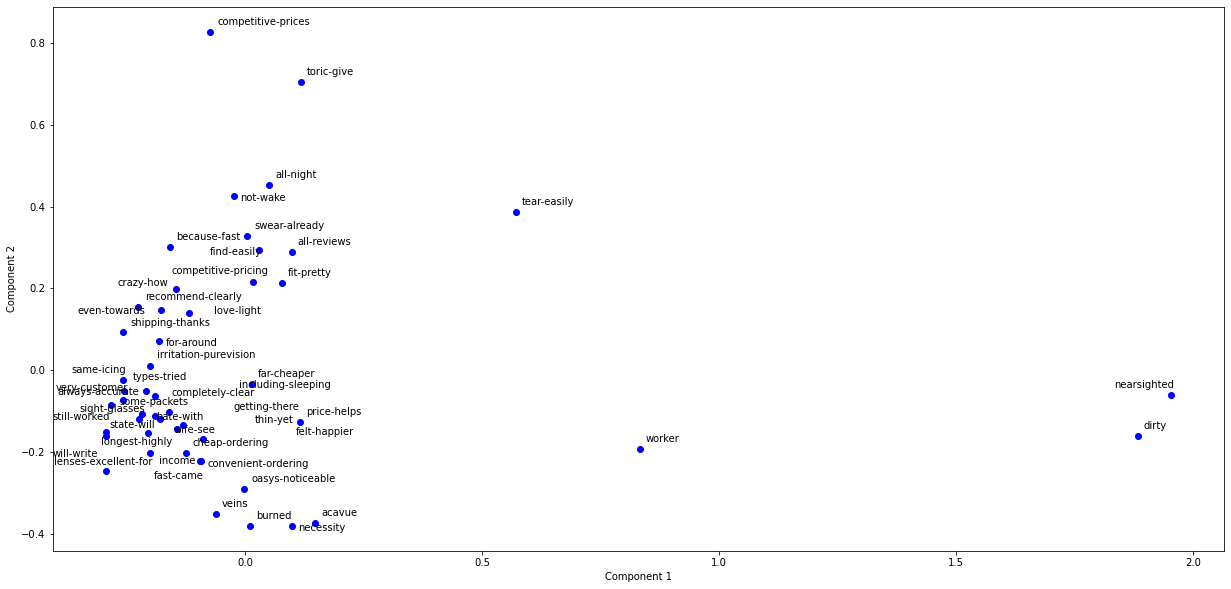
\includegraphics[width=\textwidth]{word_vec_pca.png}
         \caption{Distribution of words over all topics}
         \label{fig:pca}
     \end{figure}
It is not clear what "nearness" information could be extracted from this. More research is required to determine if words that are "near" each other are near in what sense.

\section{Exploratory Data Analysis (EDA) code and output}
The code and the output for EDA is found in the file: \verb|contacts_EDA.html|

\section{SVM based Sentiment Analysis code and output}
The code for Sentiment Analysis found in the file:\verb|contacts_SVM.html|

\section{Recurrent Neural Network (RNN) code and output}
The code for RNN Analysis found in the file:\verb|contacts_RNN.html|

\section{Word embedding and PCA analysis code and output}
The code and the output for Word embedding and PCA analysis is found in the file:\verb|contacts_PCA.html|

\section{Topic Modeling code and output}
The code for Topic Modeling found in the file:\verb|contacts_topics_modeling.html|


\end{appendices}

\end{document}



